\documentclass[12pt]{article}

\usepackage{hyperref}
\usepackage{amssymb}
\usepackage{amsfonts}
\usepackage{amsmath}
\usepackage{amscd}
\usepackage{amsthm}
\usepackage{amstext}
\usepackage{graphicx}
\usepackage{url}
\usepackage[section]{placeins}
\usepackage{caption}

\usepackage{rotating}
%\usepackage{subfig}
\usepackage{setspace}
\usepackage{lscape}
\usepackage{setspace}
\usepackage{latexsym}       % For funny characters
\usepackage{indentfirst}    % Indents all paragraphs
\usepackage{geometry}       % Increase page margins
\usepackage{epsfig}
\usepackage{yhmath}
\usepackage{footnote}
\usepackage{epic}
\usepackage{wrapfig}
%\usepackage[mdyy]{datetime}
\usepackage{booktabs}
\usepackage{pdflscape}
\usepackage{epstopdf}
\usepackage{bbm}
\usepackage{subcaption}
\usepackage{xcolor}
\usepackage{setspace}
\usepackage{soul}

%%%%%%%%%%%%%%%%%%%%%%%%%%%%%%%%%%%%%%%%%%%%%%%%%%%%%%%%%%%%%%%%%%%%%%%
\usepackage{setspace}
%\usepackage[margin=0.2in]{geometry}
\usepackage{amsmath}
\usepackage{bm}
\usepackage{mathtools}
\usepackage{amssymb}
\usepackage{lscape}
\usepackage{threeparttable}
\usepackage[utf8]{inputenc}
\usepackage{natbib}
\usepackage{lscape}
\usepackage{longtable} 
\usepackage[english]{babel}
\usepackage{graphicx}
\usepackage{color,hyperref}
\usepackage[ruled,linesnumbered]{algorithm2e}
\usepackage{dsfont}
\usepackage{mathrsfs} 
\definecolor{darkblue}{rgb}{0.0,0.0,0.3}
\hypersetup{colorlinks,breaklinks,
	linkcolor=darkblue,urlcolor=darkblue,
	anchorcolor=darkblue,citecolor=darkblue}
\usepackage{epsf}
\usepackage[font=scriptsize]{subcaption}
\captionsetup{compatibility=false}


\onehalfspacing

\setcounter{MaxMatrixCols}{10}
%TCIDATA{OutputFilter=LATEX.DLL}
%TCIDATA{Version=5.50.0.2960}
%TCIDATA{<META NAME="SaveForMode" CONTENT="1">}
%TCIDATA{BibliographyScheme=Manual}
%TCIDATA{LastRevised=Wednesday, April 01, 2015 23:48:48}
%TCIDATA{<META NAME="GraphicsSave" CONTENT="32">}
%TCIDATA{Language=American English}

\geometry {left=1in,right=1in,top=1in,bottom=1in}


%%%%%%%%%%%%%%%%%%%%%%%%%%%%%%%%%%%%%%%%%%%
%%%%%%%%%%%%%%%%%%%%%%%%%%%%%%%%%%%%%%%%%%%


%%%%%%%%%%%%%%%%%%%%%%%%%%%%%%%%%%%%%%%%%%%
%%%%%%%%%%%%%%%%%%%%%%%%%%%%%%%%%%%%%%%%%%%

\begin{document}

\noindent {\bf \large ONLINE APPENDIX for "Taxing Billionaires: Estate Taxes and the Geographical Location of the Ultra-Wealthy" by Enrico Moretti and Daniel J. Wilson -- Not For Publication}
\vspace{20pt}

\noindent {\bf \large ONLINE APPENDIX A -- Data Used in Cost-Benefit Calculations}
\vspace{10pt}

In this appendix, we discuss the data that we use in section \ref{all} to compute the costs and benefits of a broad-based estate tax on wealthy taxpayers.
We use equations (\ref{eq3}) and (\ref{eq4}).   
We need  state-by-state data or estimates on (1) the estate tax base ($(W_{as} N_{as}$) -- i.e., the total wealth of all state residents with wealth above the exemption level, (2) the income tax base for potential estate taxpayers ($(Y_{as} N_{as}$) -- i.e., the total income of all state residents with wealth above the exemption level, (3) the average effective tax rates on estate wealth ($\tau_s^{W}$) and income ($\tau_s^{Y}$) for potential estate taxpayers. 

\textbf{Estate tax base. }
In 2017, the federal estate tax applies to estate values above \$5.5 million for individuals and \$11 million for couples. Most current estate-tax states follow this federal exemption level, while some had lower exemptions. (The lowest is \$1 million in Massachusetts and Oregon (see \cite{michael2018survey}).
In our calculations, we use for simplicity the same exemption threshold  that applies U.S. federal estate tax 
and same degree of progressivity -- except with a 16\% top marginal rate, which is the top rate nearly all estate-tax states have currently. 

To estimate the potential estate tax base in each state, we start with IRS Statistics on Income (SOI) data on total estate values reported on federal estate tax returns by state of residence.\footnote{\url{https://www.irs.gov/statistics/soi-tax-stats-estate-tax-statistics-filing-year-table-2}.} Because the wealth by state on federal estate tax returns can be volatile from year to year, especially for small states, we use the average over 2015-2017 rather than just 2017. To fully utilize age-specific IRS data on income to wealth ratios discussed below, we apportion the statewide estate values to three broad age group (under 70, 70-79, and over 79) using national shares of estate tax returns by age group. Following the estate multiplier technique of \cite{kopczuk-saez:2004} and others, we estimate the underlying living population of wealthy taxpayers in each state by dividing the total estate values by the mortality rate for each age group from the Social Security Administration.\footnote{\url{https://www.ssa.gov/oact/STATS/table4c6.html}.} Given that mortality rates have been found to be considerably lower for the wealthy than for the general population, we adjust the mortality rates based on the mortality differentials provided in \cite{saez-zucman:2019}.   

\textbf{Income tax base.}
The income tax base for the population of potential estate taxpayers, by state and age group, can be estimated by multiplying the state-specific taxable estate tax values ($W_{as} N_{as}$) obtained above by the aggregate ratio of taxable income ($Y_a N_a$) to taxable estate value ($W_a N_a$) over all federal estate taxpayers:
%\begin{equation}
 $   Y_{as} N_{as} = W_{as} N_{as} \left(\frac{Y_a N_a}{W_a N_a}\right) $.
%\end{equation}
The national aggregates of $Y_a N_a$ and $W_a N_a$, by age group, are provided by the IRS Statistics on Income. Specifically, for 2008, the IRS matched all federal estate tax returns to the Form 1040 income tax returns filed by the decedent in the year prior to death. They report both taxable estate value and prior-year taxable income across taxpayers within each broad age group.\footnote{We add back spousal bequest deductions to taxable estate value because our cost estimates are based on revenues collected when the surviving spouse dies.} In aggregate, these taxpayers had taxable estate values of \$117.1 billion and prior-year taxable incomes of \$7.9 billion -- an income/wealth ratio of 0.074. The ratio falls with age (due primarily to labor income falling sharply over these three age groups): It is 0.103 for those under 70, 0.071 for ages 70 to 79, and 0.058 for those over 79.

\textbf{Average tax rates.}
For the average income tax rate, we use the top marginal tax rate, as we did in the previous section. Top income tax brackets among states generally start at incomes well below the income levels of individuals with wealth above the federal estate tax exemption (\$11 million for couples). Given that we seek to estimate the costs and benefits of states adopting an estate tax with the same degree of progressivity as the federal estate tax, albeit with a lower top rate (16\%), we need to take account of this progressivity when estimating the average effective estate tax rate. To estimate this average rate, we multiply the top marginal rate in state estate taxes, 16\%, by the ratio of the average tax rate to the top marginal tax rate in the federal estate tax. The federal top marginal rate in 2017 was 40\%. The average effective tax rate, based on 2017 IRS SOI data on total estate tax payments as a percentage of taxable estate values (adjusted for spousal deductions), was 25\%. Hence, we estimate the state average estate tax rate would be 16\%*(25/40) = 10\%.

%\textbf{Additional parameters.} For $T_a$ and $r$, we use the same parameters that we used for billionaires. 

\clearpage



%%%%%%%%%%%%%%%%%%%%%%%%%%%%%%%%%%%%%%%%%%%%%%%%%%%%%%%
% Appendix Tables and Figures
%%%%%%%%%%%%%%%%%%%%%%%%%%%%%%%%%%%%%%%%%%%%%%%%%%%%%%%
\setcounter {table} {0}
\setcounter {figure} {0}
\renewcommand{\thetable}{B\arabic{table}}
\renewcommand{\thefigure}{B\arabic{figure}}




%\graphicspath{{Figures/}}
\begin{table}
\begin{center}
\textbf{ONLINE APPENDIX B}

	\caption{\\Maximum Federal Credit Schedule for State Estate Taxes\\1954-2001}
		\scalebox{1} {
		\renewenvironment{table}[1][]{\ignorespaces}{\unskip}
        \begin{tabular}{ccc}
		Taxable Estate (\$)&Base Amount of Credit (\$)&Credit Rate on Excess (\%) \\
\midrule
100,000&0&0.8 \\
150,000&400&1.6 \\
200,000&1,200&2.4 \\
300,000&3,600&3.2 \\
500,000&10,000&4.0 \\
700,000&18,000&4.8 \\
900,000&27,600&5.6 \\
1,100,000&38,800&6.4 \\
1,600,000&70,800&7.2 \\
2,100,000&106,800&8.0 \\
2,600,000&146,800&8.8 \\
3,100,000&190,800&9.6 \\
3,600,000&238,800&10.4 \\
4,100,000&290,800&11.2 \\
5,100,000&402,800&12.0 \\
6,100,000&522,800&12.8 \\
7,100,000&650,800&13.6 \\
8,100,000&786,800&14.4 \\
9,100,000&930,800&15.2 \\
10,100,000&1,082,800&16.0 \\
\midrule

        \label{tab:fedcreditrates}
        \end{tabular}
	}
\end{center}
\vspace{-6pt}
\footnotesize{\qquad \qquad \qquad \quad Source: \cite{bakija/slemrod:2004}, Table 1}
\vspace{10cm}
\end{table}


\begin{table}
	\centering
	\caption{Probability of State Having an Estate Tax -- Linear Probability Model}
	\scalebox{0.8}{
		\renewenvironment{table}[1][]{\ignorespaces}{\unskip}
		{
\def\sym#1{\ifmmode^{#1}\else\(^{#1}\)\fi}
\begin{tabular}{l*{3}{c}}
\hline\hline
                &\multicolumn{1}{c}{(1)}&\multicolumn{1}{c}{(2)}&\multicolumn{1}{c}{(3)}\\
                &\multicolumn{1}{c}{Estate Tax Indicator}&\multicolumn{1}{c}{Estate Tax Indicator}&\multicolumn{1}{c}{Estate Tax Indicator}\\
\hline
Top PIT Rate    &  0.00697         &   0.0119         &   0.0486\sym{*}  \\
                & (0.0228)         & (0.0243)         & (0.0282)         \\
[1em]
Top Corp. Income Tax (CIT) Rate&    4.595\sym{*}  &    3.994         &    3.977         \\
                &  (2.480)         &  (2.576)         &  (3.187)         \\
[1em]
Log Change in real GDP&-0.0000390         &0.00000809         &-0.000148         \\
                &(0.000357)         &(0.000492)         &(0.000322)         \\
[1em]
Top PIT Rate X post-2001&   0.0157         &   0.0116         &  0.00390         \\
                & (0.0231)         & (0.0234)         & (0.0211)         \\
[1em]
Top CIT Rate X post-2001&   -1.116         &   -0.212         &    1.010         \\
                &  (2.749)         &  (2.919)         &  (3.066)         \\
[1em]
GDP Change X post-2001&-0.00000228         & 0.000274         & 0.000267         \\
                &(0.000224)         &(0.000610)         &(0.000620)         \\
[1em]
Constant        &   0.0496         &    0.225         &    0.213         \\
                &  (0.343)         &  (0.409)         &  (0.323)         \\
\hline
Observations    &     1333         &     1333         &     1333         \\
State Fixed Effects         &       No         &       No         &      Yes         \\
Year Fixed Effects          &       No         &      Yes         &      Yes         \\
\hline \hline
\multicolumn{3}{l}{\footnotesize Standard errors (clustered by state) in parentheses.}\\
\multicolumn{3}{l}{\footnotesize \sym{*} \(p<0.10\), \sym{**} \(p<0.05\), \sym{***} \(p<0.01\)}  \end{tabular} }

		\unskip
	}
\label{tab:ETadopt}
\end{table}
\clearpage


\begin{center}
\begin{table}
	\caption{Summary Statistics}
	\vspace{10pt}

	\begin{center}
	\caption*{Panel A. Individual-by-Year Observations. 1982 -- 2017}
	\scalebox{0.8} {
		\renewenvironment{table}[1][]{\ignorespaces}{\unskip}
		{
\def\sym#1{\ifmmode^{#1}\else\(^{#1}\)\fi}
\begin{tabular}{l*{1}{ccccc}}
\hline\hline
                    &      Mean&              Median&Standard Deviation&             Minimum&   Maximum\\
\hline
Age                 &     64.31&               65.00&     13.11&               23.00&     96.00\\
Net Worth (billions, 2017 dollars)&      3.02&                1.60&      5.73&                0.19&    125.06\\
\hline
Observations        &     13432&                    &          &                    &          \\
\hline\hline
\end{tabular}
}

		\unskip
	}
	\end{center}
	\vspace{20pt}

	\begin{center}
	\caption*{Panel B. Distribution of Net Worth -- 2017}
	\scalebox{0.8} {
		\renewenvironment{table}[1][]{\ignorespaces}{\unskip}
{
	\def\sym#1{\ifmmode^{#1}\else\(^{#1}\)\fi}
	\begin{tabular}{l*{1}{ccccccc}}
		\hline\hline
		
		
		
&1st&10th&25th&50th&75th&90th&99th \\
\midrule
Net Worth (bill)&2.0&2.2&2.7&3.7&5.5&12.0&71.0 \\
\end{tabular}


}
		
		 \unskip
           }
	   
	\end{center}
	\vspace{10pt}

	\begin{center}
	\caption*{Panel C. State-by-Year Observations.  1982 -- 2017}
	\scalebox{0.8} {
		\renewenvironment{table}[1][]{\ignorespaces}{\unskip}
		{
\def\sym#1{\ifmmode^{#1}\else\(^{#1}\)\fi}
\begin{tabular}{l*{1}{ccccc}}
\hline\hline
                    &      Mean&              Median&Standard Deviation&             Minimum&   Maximum\\
\hline
Population of Forbes 400&      7.68&                3.00&     15.07&                0.00&     98.00\\
Net Worth (billions 2017 dollars)&     22.63&                5.86&     53.36&                0.00&    617.80\\
Estate Tax Indicator&      0.32&                0.00&      0.47&                0.00&      1.00\\
Top PIT Rate        &      4.86&                5.40&      2.96&                0.00&     14.10\\
\hline
Observations        &      1750&                    &          &                    &          \\
\hline\hline
\end{tabular}
}

		\unskip
	}
	\end{center}

\label{tab:summstats}
\end{table}
\end{center}

\clearpage


\begin{table}
	\caption{Forbes 400 by Consolidated Metro Area (Top 40), 2017}
	\centering
		\scalebox{0.81} {
        \begin{tabular}{lccc}
		& Forbes Population & Mean Wealth & 1982-2017 Change\\City & in 2017& in 2017 (mil) & in Forbes Population\\
\midrule
Atlanta-Sandy Springs-Gainesville, GA-AL&9&4767&2 \\
Austin-Round Rock-Marble Falls, TX&4&8025&4 \\
Birchwood&1&4200&1 \\
Bloomington, IN&1&7500&1 \\
Boston-Worcester-Manchester, MA-RI-NH&8&5988&-2 \\
Chicago-Naperville-Michigan City, IL-IN-WI&14&3443&-2 \\
Columbia, MO&2&6800&2 \\
Dallas-Fort Worth, TX&18&5950&-9 \\
Denver-Aurora-Boulder, CO&4&9900&-1 \\
Detroit-Warren-Flint, MI&3&4400&-1 \\
Fayetteville-Springdale-Rogers, AR-MO&4&20375&3 \\
Houston-Baytown-Huntsville, TX&11&4464&-10 \\
Indianapolis-Anderson-Columbus, IN&2&2700&0 \\
Jackson, WY&4&11700&4 \\
Kalamazoo-Portage, MI&2&3950&0 \\
Knoxville-Sevierville-La Follette, TN&2&3050&2 \\
Las Vegas-Paradise-Pahrump, NV&7&7471&4 \\
Los Angeles-Long Beach-Riverside, CA&31&4806&3 \\
Miami-Fort Lauderdale-Pompano Beach, FL&25&4416&13 \\
Milwaukee-Racine-Waukesha, WI&4&3800&3 \\
Minneapolis-St. Paul-St. Cloud, MN-WI&2&4100&-5 \\
Naples-Marco Island, FL&3&5033&2 \\
Nashville-Davidson--Murfreesboro--Columbia, TN&4&4275&3 \\
New York-Newark-Bridgeport, NY-NJ-CT-PA&80&6368&-9 \\
Oklahoma City-Shawnee, OK&3&7867&-2 \\
Omaha-Council Bluffs-Fremont, NE-IA&2&41100&1 \\
Philadelphia-Camden-Vineland, PA-NJ-DE-MD&5&3500&-16 \\
Phoenix-Mesa-Glendale, AZ&5&2780&5 \\
Portland-Vancouver-Hillsboro, OR-WA&2&14450&0 \\
Raleigh-Durham-Cary, NC&2&6700&2 \\
Rochester-Batavia-Seneca Falls, NY&2&2850&2 \\
San Diego-Carlsbad-San Marcos, CA&2&3750&-2 \\
San Jose-San Francisco-Oakland, CA&54&8154&37 \\
Santa Barbara-Santa Maria-Goleta, CA&2&4250&2 \\
Seattle-Tacoma-Olympia, WA&8&29775&7 \\
St. Louis-St. Charles-Farmington, MO-IL&2&5450&1 \\
Tampa-St. Petersburg-Clearwater, FL&4&2375&3 \\
Tulsa-Bartlesville, OK&2&5350&0 \\
Washington-Baltimore-Northern Virginia, DC-MD-VA-WV&10&5490&4 \\
Average&9&7470&1 \\

        \end{tabular}
        }
\label{tab3}
\end{table}



%\begin{landscape}
\tiny{
\begin{longtable}{l l l l l l}
			\caption{State of Deaths and State of Residence Reported by Forbes}\\ 
			\hline 
		Name &Death &Death &Obituary &Forbes &Notes\\ 
		  &Year &State &Res. State &Res. State & \\ [0.5ex]
		\hline
		
		Liliore Green Rains&1985&CA&CA&CA&\\
		Mary Belin Du Pont Faulkner&1985&MA&MA&MA&\\
		Abram Nicholas Pritzker&1986&IL&&IL&\\
		David Whitmire Hearst&1986&CA&CA&CA&\\
		Gordon Barton Mclendon&1986&TX&TX&TX&\\
		Howard Vollum&1986&OR&OR&OR&\\
		Arnold Bernhard&1987&NY&NY/CT&CT&\\
		Burton Green Bettingen&1987&CA&CA&CA&\\
		Henry Ford II&1987&MI&MI&FL&\\
		Henry John Heinz II&1987&FL&PA&PA&Died at winter home.\\
		Paul Kalmanovitz&1987&CA&CA&CA&\\
		Ruth Chandler Von Platen&1987&CA&CA&CA&\\
		Sol Goldman&1987&NY&NY&NY&\\
		John Wilmer Galbreath&1988&OH&OH&OH&\\
		Lawrence Arthur Wien&1988&CT&CT/NY/FL&NY&\\
		Pierre Samuel Du Pont&1988&DE&DE&DE&\\
		Henry Crown&1990&IL&IL &IL&\\
		Mark Goodson&1992&NY&NY&NY&\\
		Edward John Debartolo&1994&OH&OH&OH&\\
		Milton Jack Petrie&1994&NY&NY&NY&\\
		Albert B Alkek&1995&TX&TX&TX&\\
		Alpheus Lee Ellis&1995&FL&FL&FL&\\
		Erskine Bronson Ingram&1995&TN&TN&TN&\\
		James Lawrence Walton&1995&AR&FL&AR&Died on fishing trip.\\
		John Jeffry Louis&1995&IL&IL&IL&\\
		Joseph R Coulter&1995&FL&FL&FL&\\
		Walter A Haas&1995& CA&CA&CA&\\
		Bob John Magness&1996&CO&VA&&UVA hospital.\\
		Daniel James Terra&1996&WA&IL/WA/France&IL&\\
		David Packard&1996&CA&CA&CA&\\
		Louis Larrick Ward&1996&MO&MO&MO&\\
		Claude Bernard Pennington&1997&LA&LA&LA&\\
		Herbert Allen&1997&NY&NY&NY&\\
		Jack Kent Cooke&1997&DC&DC&VA&\\
		Roberto Crispulo Goizueta&1997&GA&GA&GA&\\
		Betsey Cushing Roosevelt Whitney&1998&NY&NY &NY&\\
		Dwight Lyman Stuart&1998&CA&CA&CA&\\
		John William Berry&1998&OH&OH&OH&\\
		William Michael Cafaro&1998&OH&OH&OH&\\
		Curtis Leroy Carlson&1999&MN&MN&MN&\\
		Forrest Edward Mars Sr&1999&FL&FL&NV&\\
		Henry Earl Singleton&1999&CA&CA&CA&\\
		Jay Arthur Pritzker&1999&IL&IL&IL&\\
		Leon Hess&1999&NY&NY&NJ&\\
		Paul Mellon&1999&VA&VA&VA&\\
		Ruth Ray Hunt&1999&TX&TX&TX&\\
		Ted Arison&1999&Tel Aviv&Tel Aviv&FL&\\
		Bill Daniels&2000&CA&CA&CO&Died in hospital.\\
		Marshall Naify&2000&CA&CA&CA&\\
		Randolph Apperson Hearst&2000&NY&NY&NY&\\
		Edmund Wattis Littlefield&2001&CA&CA&CA&\\
		Larry Fisher&2001&FL&FL/ NY&NY&\\
		Malcom Purcell Mclean&2001&NY&NY&NY&\\
		Michel Fribourg&2001&NY&NY&NY&\\
		Reese Mcintosh Rowling&2001&TX&TX&TX&\\
		William Redington Hewlett&2001&CA&CA&CA&\\
		Alfred Lerner&2002&OH&OH&OH&\\
		Kathryn Mccurry Albertson&2002&ID&ID&ID&\\
		Millicent V Boudjakdji&2002&LA&LA&CA&\\
		Robert Henry Dedman&2002&TX&TX&TX&\\
		Victor Posner&2002&FL&FL&FL&\\
		Walter Hubert Annenberg&2002&PA&PA/CA&PA&\\
		Edward Lewis Gaylord&2003&OK&OK&OK&\\
		Joan Beverly Kroc&2003&CA&CA&CA&\\
		Laurence Alan Tisch&2003&NY&NY&NY&\\
		Samuel Jayson LeFrak&2003&NY&NY&NY&\\
		Charles B Benenson&2004&FL&NY&NY&Died suddenly.\\
		Jay Van Andel&2004&MI&MI&MI&\\
		Laurance Spelman Rockefeller&2004&NY&NY&NY&\\
		Marvin Harold Davis&2004&CA&CA&CA&\\
		Samuel Curtis Johnson&2004&WI&WI&WI&\\
		Susan Thompson Buffett&2004&CA&WY&CA&Died on vacation.\\
		Franklin Parsons Perdue&2005&MD&MD&MD&\\
		Jackson Thomas Stephens&2005&AR&AR&AR&\\
		Peter E Haas&2005&CA&CA&CA&\\
		Preston Robert Tisch&2005&NY&NY&NY&\\
		James R Cargill&2006&MN&MN&MN&\\
		Lamar Hunt&2006&TX&TX&TX&\\
		Margaret Anne Cargill&2006&CA&CA&CA&\\
		Raymond J Noorda&2006&UT&UT&UT&\\
		Robert Edward Rich&2006&FL&FL&FL&\\
		Barbara Cox Anthony&2007&HI&GA/HI&HI&\\
		Helen Walton&2007&AR&AR&AR&\\
		James Martin Moran&2007&FL&FL&FL&\\
		Margaret Hunt Hill&2007&TX&TX&TX&\\
		James LeVoy Sorenson&2008&UT&UT&UT&\\
		John Hugh Macmillan&2008&FL&FL&FL&\\
		John Richard Simplot&2008&ID&ID&ID&\\
		Carl Ray Pohlad&2009&MN&MN&MN&\\
		Frank Batten&2009&VA&VA&VA&\\
		Melvin Simon&2009&IN&IN&IN&\\
		Samuel J Heyman&2009&NY&NY, FL, CN&NY&Died after surgery.\\
		Trammell Crow&2009&TX&TX&TX&\\
		William Morse Davidson&2009&MI&MI&MI&\\
		Dolph Briscoe&2010&TX&TX&TX&\\
		John Werner Kluge&2010&VA&VA&FL&\\
		Paul Milstein&2010&NY&NY&NY&\\
		Richard N Goldman&2010&CA&CA&CA&\\
		Cargill Macmillan&2011&CA&CA&CA&\\
		Carl Henry Lindner&2011&OH&OH&OH&\\
		Jack N Mandel&2011&OH&OH&OH&\\
		Jean Ellen Du Pont Sheehan&2011&DE&DE&FL&\\
		John Charles Haas&2011&PA&PA&PA&\\
		John Edward Anderson&2011&CA&CA&CA&\\
		Malcolm Green Chace&2011&MA&MA&RI&\\
		Robert Alan Pritzker&2011&IL&IL&IL&\\
		William Alfred Cook&2011&IN&IN&IN&\\
		Albert Lee Ueltschi&2012&FL&FL&FL&\\
		Donald J Schneider&2012&WI&WI&WI&\\
		Barbara Piasecka Johnson&2013&Poland&Italy, Poland, Monaco&NJ&\\
		Edgar Miles Bronfman&2013&NY&NY&NY&\\
		Harold Clark Simmons&2013&TX&TX&TX&\\
		Leonard Samuel Skaggs&2013&UT&UT&UT&\\
		Robert Earl Holding&2013&UT&&ID&Res. state unclear.\\
		James Edwards Stowers&2014&MO&MO&MO&\\
		Malcolm Glazer&2014&FL&FL&FL&\\
		Nelson Bunker Hunt&2014&TX&TX&TX&\\
		Patrick Joseph Mcgovern&2014&NH&CA&NH&\\
		Kirk Kerkorian&2015&CA&CA&CA&\\
		Michael Birck&2015&IL&IL&IL&\\
		Ralph J Roberts&2015&PA&PA&PA&\\
		Forrest Edward Mars Jr&2016&WY&WA&WY&\\
		Jack Crawford Taylor&2016&MO&MO&MO&\\
		Joseph C Mandel&2016&FL&OH&OH&Died at winter home.\\
		Leandro Rizzuto&2017&FL&FL&WY&\\
		Michael Ilitch&2017&MI&MI&MI&\\
		Samuel Irving Newhouse&2017&NY&NY&NY&\\
		Charles B Wang&2018&NY&NY&NY&\\
		\hline
\label{deaths}
\end{longtable}
%\end{landscape}
}	

\clearpage


\begin{table}
\centering
	\caption{Robustness}
%	\vspace{4pt}
	\caption*{Panel A. Difference-in-Difference}
	\scalebox{0.8} {
		\renewenvironment{table}[1][]{\ignorespaces}{\unskip}
		{
\def\sym#1{\ifmmode^{#1}\else\(^{#1}\)\fi}
\begin{tabular}{l*{4}{c}}
\hline\hline
                &\multicolumn{1}{c}{(1)}&\multicolumn{1}{c}{(2)}&\multicolumn{1}{c}{(3)}&\multicolumn{1}{c}{(4)}\\
                &\multicolumn{1}{c}{Top 100}&\multicolumn{1}{c}{Top200}&\multicolumn{1}{c}{Top300}&\multicolumn{1}{c}{10+ Obs}\\
\hline
ET-state X post-2001&   -0.553\sym{***}&   -1.307\sym{***}&   -1.902\sym{***}&   -2.182\sym{***}\\
                &  (0.105)         &  (0.195)         &  (0.388)         &  (0.522)         \\
[1em]
ET-state        &   0.0599         &    0.500         &    0.911\sym{*}  &    0.944\sym{***}\\
                &  (0.199)         &  (0.318)         &  (0.466)         &  (0.356)         \\
\hline
Observations    &     1575         &     1610         &     1680         &     1575         \\
Semi-elasticity            &    -.338         &    -.327         &    -.361         &      -.4         \\
\quad \textit{Std. Error}          &     .064         &     .049         &     .073         &     .096         \\
\hline \hline
\multicolumn{5}{l}{\footnotesize Driscoll-Kraay (with 10-year bandwidth) standard errors in parentheses.} \\
\multicolumn{5}{l}{\footnotesize All regressions include state and year fixed effects.} \\
\multicolumn{5}{l}{\footnotesize \sym{*} \(p<0.10\), \sym{**} \(p<0.05\), \sym{***} \(p<0.01\)}  \end{tabular} }

	}
	
%	\vspace{4pt}
	\caption*{Panel B. Triple-Difference}
	\scalebox{0.8} {
		\renewenvironment{table}[1][]{\ignorespaces}{\unskip}
		{
\def\sym#1{\ifmmode^{#1}\else\(^{#1}\)\fi}
\begin{tabular}{l*{4}{c}}
\hline\hline
                &\multicolumn{1}{c}{(1)}&\multicolumn{1}{c}{(2)}&\multicolumn{1}{c}{(3)}&\multicolumn{1}{c}{(4)}\\
                &\multicolumn{1}{c}{Top 100}&\multicolumn{1}{c}{Top200}&\multicolumn{1}{c}{Top300}&\multicolumn{1}{c}{10+ Obs}\\
\hline
ET-state X post-2001 X old&   -0.762\sym{***}&   -0.808\sym{***}&   -1.127\sym{***}&   -1.178\sym{**} \\
                &  (0.166)         &  (0.265)         &  (0.346)         &  (0.471)         \\
[1em]
ET-state X old  &    0.245\sym{***}&    0.272\sym{***}&    0.411\sym{***}&    0.440\sym{**} \\
                & (0.0779)         & (0.0749)         & (0.0990)         &  (0.188)         \\
[1em]
ET-state X post-2001&    0.104         &   -0.250\sym{*}  &   -0.388\sym{**} &   -0.502\sym{**} \\
                & (0.0842)         &  (0.130)         &  (0.152)         &  (0.240)         \\
[1em]
old X post-2001 &    0.893\sym{***}&    1.181\sym{***}&    1.603\sym{***}&    2.166\sym{***}\\
                &  (0.121)         &  (0.242)         &  (0.301)         &  (0.537)         \\
[1em]
ET-state        &  -0.0926         &    0.114         &    0.250         &    0.252         \\
                & (0.0888)         &  (0.147)         &  (0.224)         &  (0.194)         \\
[1em]
old             &   -0.206\sym{***}&   -0.352\sym{***}&   -0.499\sym{***}&   -0.459\sym{*}  \\
                & (0.0586)         & (0.0843)         &  (0.149)         &  (0.244)         \\
\hline
Observations    &     3150         &     3220         &     3360         &     3150         \\
Semi-elasticity, Young      &     .036         &    -.086         &    -.133         &    -.173         \\
\quad \textit{Std. Error}    &     .029         &     .045         &     .052         &     .083         \\
Semi-elasticity, Old        &    -.603         &    -.465         &     -.49         &    -.499         \\
\quad \textit{Std. Error}      &     .101         &     .085         &     .108         &      .13         \\
\hline \hline
\multicolumn{5}{l}{\footnotesize Driscoll-Kraay (with 10-year bandwidth) standard errors in parentheses. All regressions} \\
\multicolumn{5}{l}{\footnotesize include year fixed effects. State fixed effects are absorbed by old-young differencing.} \\
\multicolumn{5}{l}{\footnotesize \sym{*} \(p<0.10\), \sym{**} \(p<0.05\), \sym{***} \(p<0.01\)}  \end{tabular} }

	}

%	\vspace{4pt}
	\caption*{Panel C. Linear Probability Model}
	\scalebox{0.8} {
		\renewenvironment{table}[1][]{\ignorespaces}{\unskip}
		{
\def\sym#1{\ifmmode^{#1}\else\(^{#1}\)\fi}
\begin{tabular}{l*{4}{c}}
\hline\hline
                &\multicolumn{1}{c}{(1)}&\multicolumn{1}{c}{(2)}&\multicolumn{1}{c}{(3)}&\multicolumn{1}{c}{(4)}\\
                &\multicolumn{1}{c}{Top 100}&\multicolumn{1}{c}{Top200}&\multicolumn{1}{c}{Top300}&\multicolumn{1}{c}{10+ Obs}\\
\hline
Age X post-2001 & -0.00563\sym{***}& -0.00362\sym{***}& -0.00295\sym{***}& -0.00337\sym{***}\\
                &(0.000899)         &(0.000806)         &(0.000719)         &(0.000848)         \\
[1em]
Age             &  0.00273\sym{***}&  0.00127\sym{**} & 0.000987\sym{*}  &  0.00134\sym{**} \\
                &(0.000914)         &(0.000632)         &(0.000565)         &(0.000653)         \\
\hline
Observations    &     3276         &     6465         &     9686         &     9714         \\
\hline \hline
\multicolumn{5}{l}{\footnotesize Driscoll-Kraay standard errors in parentheses.} \\
\multicolumn{5}{l}{\footnotesize All regressions include state and year fixed effects.} \\
\multicolumn{5}{l}{\footnotesize \sym{*} \(p<0.10\), \sym{**} \(p<0.05\), \sym{***} \(p<0.01\)}  \end{tabular} }

	}
\label{tab:RestrictedSamples}
\end{table}

\clearpage

\begin{table}
	\centering
	\caption{Cost-Benefit Results Under Alternative Assumptions}
	\caption*{Panel A: Billionaires Estate Tax}
	\scalebox{0.9} {
		\renewenvironment{table}[1][]{\ignorespaces}{\unskip}
		% matrix: R1 file: ../Tables/TableB7_a.tex  15 Dec 2021 15:33:16
\begin{table}[htbp]
\begin{tabular}{|l|c|c|c|c|c|c|}\hline  
 & Baseline  & Alt 1  & Alt 2  & Alt 3  & Alt 4  & Alt 5  \\ \hline  
ET States (10) &   . &   . &   . &   . &   . &   . \\ \hline 
Average CB ratio & 0.49 & 0.18 & 0.73 & 0.41 & 0.58 & 0.23 \\ \hline 
Number with CB$\geq$1 & 1.00 & 0.00 & 2.00 & 0.00 & 1.00 & 0.00 \\ \hline 
r4 &   . &   . &   . &   . &   . &   . \\ \hline 
Non-ET States (28) &   . &   . &   . &   . &   . &   . \\ \hline 
Average CB ratio & 0.31 & 0.13 & 0.48 & 0.27 & 0.35 & 0.14 \\ \hline 
Number with CB$\geq$1 & 1.00 & 0.00 & 1.00 & 0.00 & 1.00 & 0.00 \\ \hline 
Average CB ratio &   . &   . &   . &   . &   . &   . \\ \hline 
Number with CB$\geq$1 &   . &   . &   . &   . &   . &   . \\ \hline 
r10 & 0.36 & 0.14 & 0.55 & 0.31 & 0.42 & 0.17 \\ \hline 
All States (38) & 2.00 & 0.00 & 3.00 & 0.00 & 2.00 & 0.00 \\ \hline 
  \end{tabular}
\end{table}

		\unskip
	}
	\vspace{10pt}
	\caption*{Panel B: Broad Estate Tax}
	\scalebox{0.9} {
		\renewenvironment{table}[1][]{\ignorespaces}{\unskip}
		% matrix: R2 file: ../Tables/TableB7_b.tex  15 Dec 2021 15:33:16
\begin{table}[htbp]
\begin{tabular}{|l|c|c|c|c|c|c|}\hline  
 & Baseline  & Alt 1  & Alt 2  & Alt 3  & Alt 4  & Alt 5  \\ \hline  
ET States (14) &   . &   . &   . &   . &   . &   . \\ \hline 
Average CB ratio & 0.71 & 0.28 & 1.05 & 0.61 & 0.83 & 0.71 \\ \hline 
Number with CB$\geq$1 & 3.00 & 0.00 & 9.00 & 1.00 & 5.00 & 3.00 \\ \hline 
r4 &   . &   . &   . &   . &   . &   . \\ \hline 
Non-ET States (36) &   . &   . &   . &   . &   . &   . \\ \hline 
Average CB ratio & 0.45 & 0.18 & 0.66 & 0.38 & 0.52 & 0.45 \\ \hline 
Number with CB$\geq$1 & 1.00 & 0.00 & 5.00 & 1.00 & 1.00 & 1.00 \\ \hline 
Average CB ratio &   . &   . &   . &   . &   . &   . \\ \hline 
Number with CB$\geq$1 &   . &   . &   . &   . &   . &   . \\ \hline 
r10 & 0.53 & 0.21 & 0.78 & 0.45 & 0.62 & 0.53 \\ \hline 
All States (50) & 4.00 & 0.00 & 14.00 & 2.00 & 6.00 & 4.00 \\ \hline 
  \end{tabular}
\end{table}

		\unskip
	}
\label{tab:CBrobustness}
\end{table}

{\footnotesize \noindent Notes: Cost-benefit ratios in Panel A exclude states that had no Forbes 400 billionaires in 2017. Baseline assumptions are described in the text. Alternative 1 assumes that wealth and income grow at 7.0\% (vs. 0\% in baseline) per year beyond 2017; 7.0\% is the average annual growth rate of Forbes 400 real wealth from 1982--2017. Alternative 2 assumes surviving spouse is 20 (vs. 10) years younger than decedent. Alternative 3 assumes states discount using a real interest rate of 1\% (vs. 2\%). Alternative 4 assumes states discount using a real interest rate of 3\%. Alternative 5, following \cite{saez-zucman:2019}, assumes income of Forbes 400 is half of income reported by top 400 income taxpayers according to IRS SOI data (vs. assuming it is 10.3\% of Forbes 400 taxable wealth). All other parameter assumptions are the same as in the baseline scenario.}

\clearpage




\begin{landscape}
\begin{figure}
    \caption{Distribution of Top Personal Income Tax Rates by State Estate Tax Status}
    \label{fig:PIT_dist}
		\begin{center}
			\begin{tabular}{@{}cc@{}cc@{}}
				
				\begin{subfigure}{0.7\textwidth}
					\caption{2001, Non-Estate Tax States}	
					\includegraphics[height=75mm]{../Figures/FigureB1_a.pdf}
				\end{subfigure} &
				\vspace{10pt}

				\begin{subfigure}{0.7\textwidth}
					\caption{2001, Estate Tax States}
					\includegraphics[ height=75mm]{../Figures/FigureB1_b.pdf}
				\end{subfigure} \\
				
				\begin{subfigure}{0.7\textwidth}
					\caption{2017, Non-Estate Tax States}
					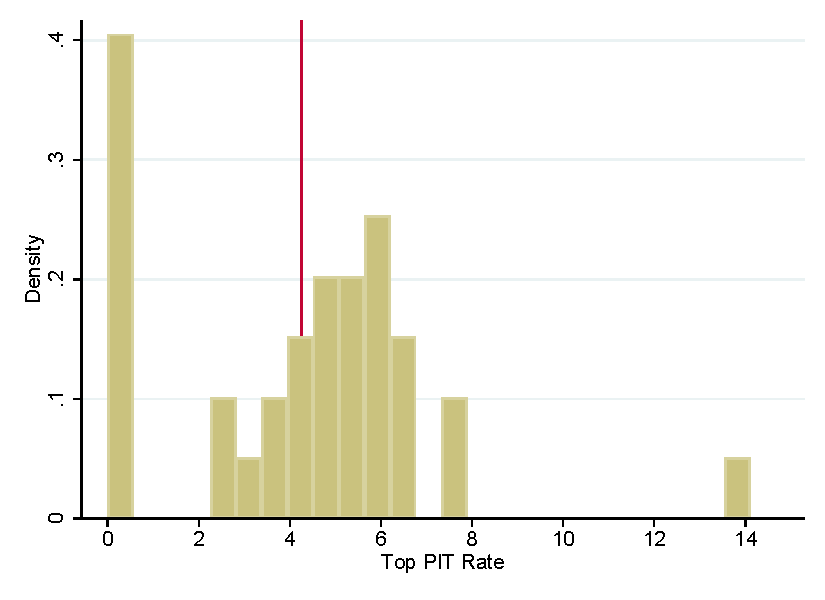
\includegraphics[ height=75mm]{../Figures/FigureB1_c.pdf}
				\end{subfigure} &
				
				\begin{subfigure}{0.7\textwidth}
					\caption{2017, Estate Tax States}
					\includegraphics[height=75mm]{../Figures/FigureB1_d.pdf}
				\end{subfigure} \\	
			\end{tabular}
		\end{center}	
{Note: red lines indicate means.}
\end{figure}
\end{landscape}
\clearpage






\begin{figure}
	\centering
	\caption{Average Wealth of Forbes 400 Sample (1982 to 2017)}
	\label{fig:avg_wealth_tsgraph}
	\includegraphics[width=1\textwidth]{../Figures/FigureB2.pdf}
	\caption*{\footnotesize *Based on our sample of Forbes 400 individual-year observations, which excludes those with no data on age or state of residence.}
\end{figure}
\clearpage




\begin{figure}
\centering
\caption{Robustness to Dropping Individual ET States}
\label{newtab33}
	\caption*{Panel A. Difference-in-Difference}
	\includegraphics[width=.7\textwidth]{../Figures/FigureB3_a.pdf}
	\caption*{Panel B. Triple-Difference}
	\includegraphics[width=.7\textwidth]{../Figures/FigureB3_b.pdf}
	\caption*{\footnotesize Notes: Panel A shows the estimated coefficient on EIxPost, and its 95\% confidence interval, from the difference-in-difference specification discussed in Section 5.1 dropping, one by one, each state that had an estate tax at some point after 2001. The leftmost coefficient, labeled ``None'', corresponds the baseline estimate shown in Table 2. Point B shows the estimated coefficient on EIxPostxOld, and its 95\% confidence interval, from the triple-difference specification discussed in Section 5.2 dropping, one by one, each state that had an estate tax at some point after 2001. The leftmost coefficient, labeled ``None'', corresponds the baseline estimate shown in Table 3.}
\end{figure}


\begin{figure}
\centering
\caption{Probability of living in High Income Tax State By Age}
	\caption*{Panel A. 1982-2001}
	\includegraphics[width=.75\textwidth]{../Figures/FigureB4_a.pdf}
	\caption*{Panel B. 2005-2017}
	\includegraphics[width=.75\textwidth]{../Figures/FigureB4_b.pdf}
	\caption*{\footnotesize Notes: Age Groups below 40 are excluded. Individuals above 95 are pooled and displayed at Age 96.}
\label{fig:figa1}
\end{figure}
\clearpage



\begin{figure}
\centering
\caption{Number of Federal Estate Taxpayers by State, 2017}
\label{new8map}
	\includegraphics[width=.99\textwidth]{../Figures/FigureB5.pdf}
	\caption*{\footnotesize Source: IRS Statistics on Income.}
\end{figure}
\clearpage



%%%%%%%%%%%%%%%%%%%%%%%%%%%%% NEW MATERIAL TO BE POTENTIAL ADDED TO THE DRAFT %%%%%%%%%%%%%%%%%%%%%%%%%%%%%%%%%%%%%%%%
\if0

\setcounter {table} {0}
\setcounter {figure} {0}
\renewcommand{\thetable}{C\arabic{table}}
\renewcommand{\thefigure}{C\arabic{figure}}



\begin{figure}
\centering
\caption{Forbes 400 Age Distribution, 1982-2017}
	\includegraphics[width=.99\textwidth]{../tables/hist_age.pdf}
\end{figure}


\begin{landscape}
\begin{table}
	\caption{Triple-Difference\\Dependent Variable: Population of Forbes 400}
	\caption*{``Old'' = 60+}
	\centering
	\scalebox{0.65} {
		\renewenvironment{table}[1][]{\ignorespaces}{\unskip}
		\input{../archive/stock_EI_old2001with060.tex}
	}
\end{table}
\clearpage

\begin{table}
	\caption{Triple-Difference\\Dependent Variable: Population of Forbes 400}
	\caption*{``Old'' = 70+ (65-69 year-olds dropped)}
	\centering
	\scalebox{0.65} {
		\renewenvironment{table}[1][]{\ignorespaces}{\unskip}
		\input{../archive/stock_EI_old2001with070.tex}
	}
\end{table}
\clearpage

\begin{table}
	\caption{Triple-Difference\\Dependent Variable: Population of Forbes 400}
	\caption*{``Old'' = 75+ (65-74 year-olds dropped)}
	\centering
	\scalebox{0.65} {
		\renewenvironment{table}[1][]{\ignorespaces}{\unskip}
		\input{../archive/stock_EI_old2001with075.tex}
	}
\end{table}
\clearpage
\end{landscape}

\fi


\end{document}





%%%%%%%%%%%%%%%%%%%%%%%%%%%%%%%%%%%%%%%%%%%%%%%%%%%%%%%%%%%%%%%
%%%%%%%%%%%%%%%%%%%%%%%%%%%%%%%%%%%%%%%%%%%%%%%%%%%%%%%%%%%%%%%
%%%%%%%%%%%%%%%%%%%%%%%%%%%%%%%%%%%%%%%%%%%%%%%%%%%%%%%%%%%%%%%
%%%%%%%%%%%%%%%%%%%%%%%%%%%%%%%%%%%%%%%%%%%%%%%%%%%%%%%%%%%%%%%
\begin{landscape}
\begin{table}
	\centering
	\caption{Probability of Moving Away from ET States and to Non-ET States}
	\caption*{Panel A: All Forbes 400 Individuals Observed in 2001}
	\scalebox{0.9} {
		\renewenvironment{table}[1][]{\ignorespaces}{\unskip}
		\input{../archive/mover_table1.tex}
		\unskip
	}
	\vspace{10pt}
	\caption*{Panel B: Forbes 400 Individuals Observed in 2001 -- 65 and Over}
	\scalebox{0.9} {
		\renewenvironment{table}[1][]{\ignorespaces}{\unskip}
		\input{../archive/mover_table2.tex}
		\unskip
	}
	\vspace{10pt}
	\caption*{Panel C: Forbes 400 Individuals Observed in 2001 -- Under 65}
	\scalebox{0.9} {
		\renewenvironment{table}[1][]{\ignorespaces}{\unskip}
		\input{../archive/mover_table3.tex}
		\unskip
	}
\label{tab:movers_table}
\end{table}

{\footnotesize Notes: ``ET'' denotes status of living in estate tax state; ``Non-ET'' denotes status of living in non-estate tax state. Sample for each column consists of Forbes 400 billionaires observed in both 2001 and year \textit{t}. Second row of each panel shows the percentage of individuals observed in 2001 who, by year \textit{t}, have physical moved from an ET state to a non-ET state. Third row of each panel shows the percentage of individuals observed in 2001 who, by year \textit{t}, have physical moved from a non-ET state to an ET state. Age is measured in 2001.}
\end{landscape}

\clearpage
